% Mẫu đề tự luận có gợi ý từng bước (\begin{huongdan}). Mỗi \buocgiai hoặc sơ đồ là một gợi ý học sinh mở bằng XP; không có lời giải chi tiết cho học sinh.
\chude{Đề thi thử tự luận HK1}

\man{1}{Đề}
\begin{extl}
Cho hình thang cân $ABCD$ ($AB\parallel CD$). Chứng minh $\widehat{ACD}=\widehat{BDC}$.
\begin{huongdan}
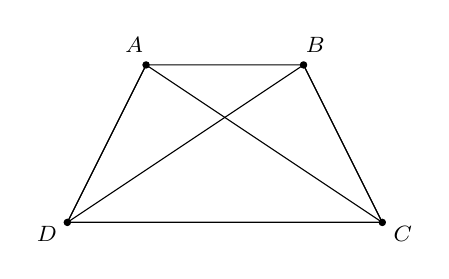
\begin{tikzpicture}[line join=round]
\coordinate (A) at (1,2); \coordinate (B) at (3,2); \coordinate (C) at (4,0); \coordinate (D) at (0,0);
\draw (A)--(B)--(C)--(D)--cycle;
\foreach \p/\g in {A/120,B/60,C/-30,D/210} \draw[fill=black] (\p) circle (.04) +(\g:.3) node[font=\footnotesize]{$\p$};
\sang{1}{\draw (A)--(C)--(D)--cycle;}
\sang{2}{\draw (B)--(D)--(C)--cycle;}
\end{tikzpicture}
\buocgiai{Chọn hai tam giác}{Xét $\triangle ACD$ và $\triangle BDC$.}{Hai góc cần so sánh nằm trong hai tam giác này.}
\buocgiai{Tìm ba yếu tố bằng nhau}{$CD$ chung, $AD=BC$, $\widehat{ADC}=\widehat{BCD}$.}{Tính chất của hình thang cân.}
\begin{sodo}
\nut{1}{$\widehat{ACD}=\widehat{BDC}$}{}
\nut{2}{$\triangle ACD=\triangle BDC$}{c.g.c}
\nut{3}{$AD=BC$, $\widehat{ADC}=\widehat{BCD}$}{hình thang cân}
\end{sodo}
\end{huongdan}
\loigiai{Lời giải cho giáo viên (học sinh không thấy).}
\end{extl}
